\chapter{Application Architecture}\label{chapter:application_architecture}
\todoin{Next few pages should describe the architecture of your solution including UML diagrams, interaction with other systems and dependencies on external libraries}
The \gnb{} application was built using a PHP backend and a web-based (HTML + Javascript) frontend. Also, the solution may provide the clients of \gnb{} with an additional SCS (short for SmartCardSimulator) software, which is needed to provide 2-step authentication during transactions and can be used on any system that supports Java 1.7+.\newline
The application was almost entirely developed without the aid of external libraries, preferring the use of builtin APIs and a custom architecture. Here is a list of the used libraries, which will be later on described more in details, along with their interaction with the system:
\begin{itemize}
	\item PHPMailer (see \texttt{https://github.com/PHPMailer/PHPMailer})
	\item fpdf (see \texttt{http://www.fpdf.org/})
	\item pdf encryption script using fpdf (see \texttt{http://www.fpdf.org/en/script/script37.php})
	\item secureimage (see \texttt{https://github.com/dapphp/securimage})
\end{itemize}

In the following section we will discuss the architecture of the whole web application; we will also provide dedicated sections for a more detailed analysis of the Entity-Relationship model used in the database as well as the architecture of the Smart Card Simulator.
\section{Architecture}

\section{Database Schema}\label{section:db}
\begin{figure}[h!tbp]
	\centering
	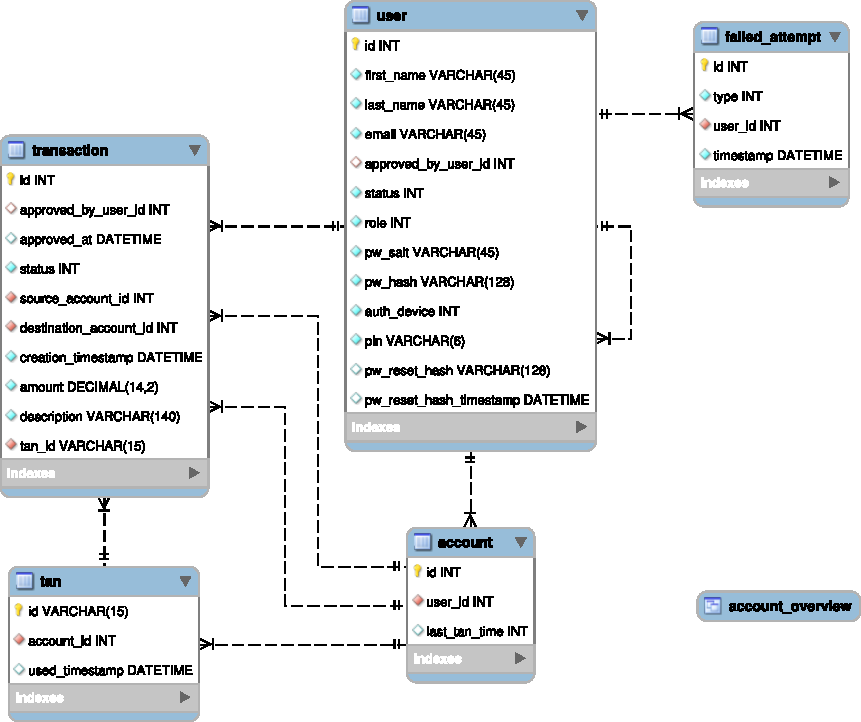
\includegraphics[width=\textwidth]{figures/database_model}
	\caption{Database model}
	\label{figure:dbmodel}
\end{figure}

The database schema was created using the \emph{MySQL Workbench}. The database schema is shown in \autoref{figure:dbmodel} and describes the following 6 entities:
\begin{description}
	\item[Table "user"] \hfill \\
	Contains all the user attributes including user ID, full name, mail, status (\texttt{unapproved}, \texttt{approved}, \texttt{rejected}, \texttt{blocked}), role (\texttt{client}, \texttt{employee}), salt and hash for the authentication, the device used for TAN authentication (\texttt{none} for users without account, otherwise \texttt{TANs} or the \texttt{SCS}), the PIN as well as the password reset hash and creation timestamp for this hash. Additionally the user ID is stored which approved/blocked/rejected the user the last time.
	
	\item[Table "account"] \hfill \\
	Contains the account number, the user ID of the owner and the timestamp of the last TAN that was used if the user is using the SCS (see \autoref{section:scs}).
	
	\item[Table "transaction"] \hfill \\
	Contains information about the status (\texttt{unapproved}, \texttt{approved}, \texttt{rejected}), the user ID of the approving/rejecting user and approval/rejection time of the transactions as well as the source and destination account, creation timestamp, amount and description of the transaction as well as the used TAN (if the SCS was not used).
	
	\item[Table "tan"] \hfill \\
	Contains the TANs and which account they belong to as well as a field specifying if the given TAN has been used (value is a timestamp) or not used (value is \texttt{NULL}).
	
	\item[Table "failed\_attempt"] \hfill \\
	Contains all failed attempts (e.g. failed \texttt{login} or invalid \texttt{tan}) and their timestamp associated to the user ID that attempted the action.
	
	\item[View "account\_overview"] \hfill \\
	Is used to obtain the balance for a given account number. As shown in \autoref{figure:accountoverviewfigure} this approach is not trivial. First (lines 8-9) we set Barney's balance to a fixed amount because all the welcome credits to new users are coming from his account. Then we exclude some transactions from our calculation, namely rejected transactions, unapproved transactions and transactions that have the same source- and destination account number (see lines 12-14). After that we determine the sign of the transaction --- it is either positive if the given account is the destination account, or negative if our account is the source account (see lines 17-19).
	
\begin{figure}[h!tbp]
	\centering
	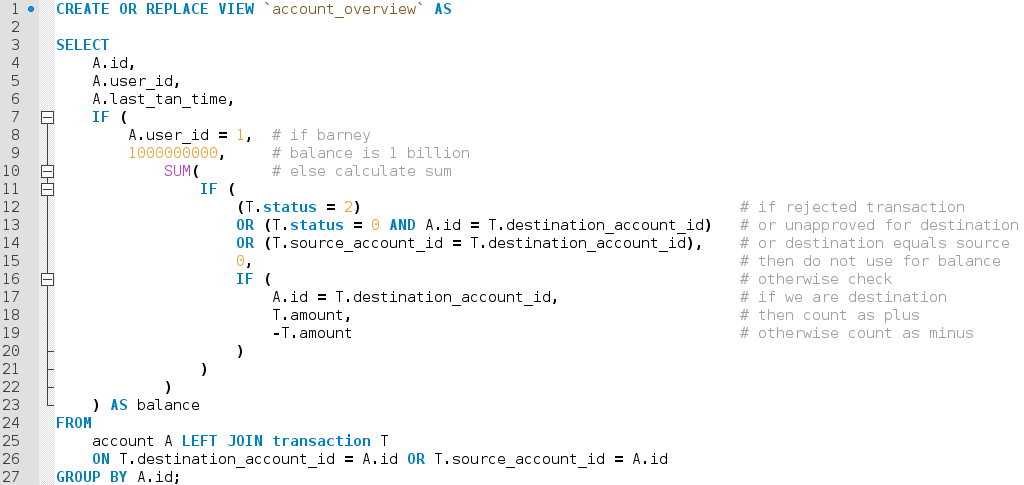
\includegraphics[width=\textwidth]{figures/code_account_overview}
	\caption{View "account\_overview"}
	\label{figure:accountoverviewfigure}
\end{figure}

\end{description}

\section{Smart Card Simulator}\label{section:scs}
The SCS is a stand-alone Java application that can be downloaded as a \texttt{.jar} file via the web application without having to be logged in as a user, i.e. the SCS is free for anyone, although only clients of the bank can make use of it. This is because the SCS allows users to generate TANs on the fly when performing transactions, instead of reading pre-generated TANs from a finite list. \newline
The \gnb{} Smart Card Simulator does not require any kind of direct interaction with the PHP backend when used, hence clients can even run it from a machine disconnected from the internet and/or different than the one they are performing the transaction from. Also, the executable file is not bound to a specific account and could, therefore, be used by multiple clients as well (or for multiple accounts).
\subsection{Usage}
When using the SCS, users are required to insert their personal PIN and all details regarding a specific transaction (either manually or contained in a batch file). The SCS will then generate a pseudo-random TAN based on the user's input and a timestamp; the web application will challenge the client to input the same data inside the transaction HTML form as well, validating it against the generated TAN. In case the TAN is proved to be invalid, the transaction fails; this is either due to a user not inserting the same values inside the SCS and the transaction page, or the user providing an invalid PIN inside the application.\newline

\begin{figure}[h!tbp]
	\centering
	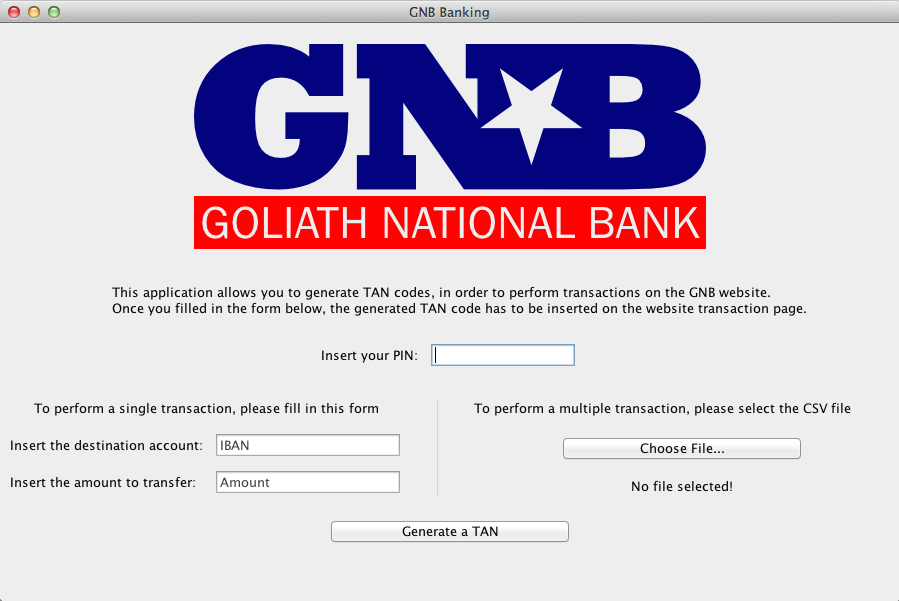
\includegraphics[width=\textwidth]{figures/scs_gui.png}
	\caption{Graphical User Interface of the SmartCard Simulator}
	\label{figure:scs_gui}
\end{figure}

\subsection{Architecture}
The solution includes the minimal amount of features required for the functionality to work. By doing so, we kept a clean and simple design, based on an MVP pattern (the architecture can be seen in \autoref{figure:scs_uml}). We will now briefly describe the architecture and the involved components.\newline
$\bullet$ The \textbf{MainView} class captures user actions callbacks and dispatches them to the Presenter class, which acts as the controller of the whole application. The view was created via a GUI Builder, using Java Swing graphical components.\newline
Event listeners are created inline inside the \texttt{initComponents} private method and associated to some objects, like the \texttt{generateButton}. When choosing to generate a TAN, the \texttt{performGenerateTan} method is automatically called within the MainView, which will retrieve the user's input and call the appropriate method inside the presenter component, depending whether the user wants to perform a batch transaction or a single transaction.\newline
Upon a successful operation, the generated TAN will be displayed by the MainView, otherwise an error will be shown to the user.\newline
$\bullet$ The \textbf{Presenter} is in charge of the business logic. When a TAN generation request is dispatched to the presenter, this component checks the validity of all user input (or the contents of the batch file) and prepares it for being processed by the CustomTanGenerator class. After CustomTanGenerator has processed the data and generated a TAN, the presenter will take care of returning it to the MainView.
Since the application does not involve a real model, the only data which can be retrieved is given by the user's input.\newline
$\bullet$ \textbf{CustomTanGenerator} is accessed statically by the presenter, as it contains only the algorithm used to generate a TAN given some input parameters. This class does not need to keep any state and will directly return the generated TAN.

\begin{figure}[h!tbp]
	\centering
	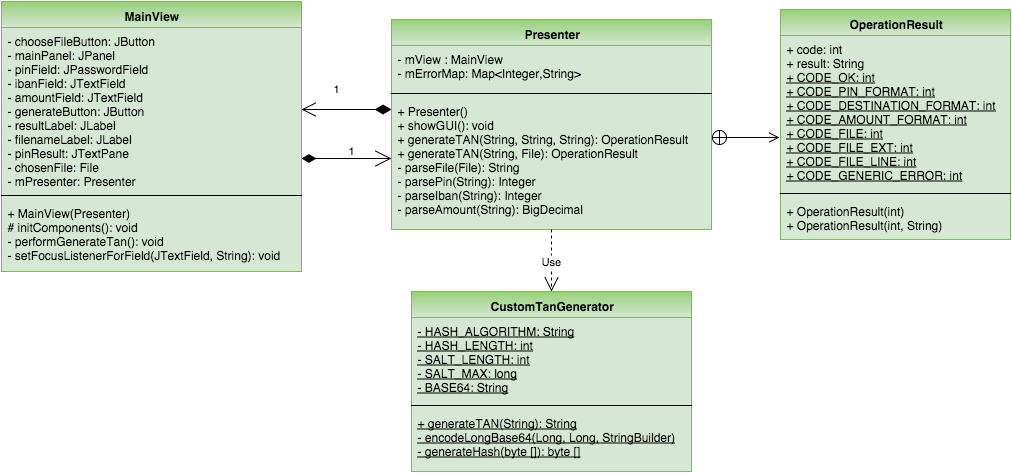
\includegraphics[width=\textwidth]{figures/scs_uml.png}
	\caption{Architecture of the SmartCard Simulator}
	\label{figure:scs_uml}
\end{figure}


\subsection{Security considerations}
As for any public cryptographic algorithm, the only thing that should be kept private is the secret shared between the client and the server, in this case being the PIN code, therefore the SCS application was not obfuscated in any way. This is also due to the overall low difficulty in reverse-engineering compiled Java code.\newline
The chosen solution is considered to be secure, as the input parameters (namely the batch transaction file or the details of a specific transaction) are hashed with a SHA-256 algorithm, together with the PIN of the user and a timestamp. 
The purpose of the timestamp is to add a degree of randomness inside the resulting TAN and avoiding replay attacks (the backend stores the time of the last transaction performed by a user). Although the timestamp can easily be guessed by an attacker, all the other values are strictly related to a specific transaction, and a brute-force attack would require a huge amount of attempts to either find a hash collision or the correct values. The \gnb{} application also provides a lockout mechanism in case a malicious attacker attempted to brute-force a TAN on the transaction page, locking him out indefinitely.\newline
Since the SCS application does not connect to the Internet in any way and the user is required to manually copy/paste a generated TAN inside the transaction page, an attacker would have to obtain complete access on the victim's machine, in order to obtain a valid TAN code and eventually brute-force the PIN. Since this is highly unlikely and in any case not due to the design of the application, the SmartCard Simulator can be considered secure.